
\subsection{Szwarc-Boryczka Algorithm}

\begin{frame}
    \frametitle{Szwarc-Boryczka Algorithm \cite{szwarc_novel_2022}}

    \note<1->[item]{
        Solution Vectors: \begin{itemize}
            \item Paths as list of nodes \begin{itemize}
                      \item Means that they can be different sizes
                  \end{itemize}
        \end{itemize}
    }
    \note<2->[item]{
        Objective function: \begin{itemize}
            \item Path Score
        \end{itemize}
    }

    \begin{itemize}
        \item<1-> Solution Vectors $\Rightarrow$ List of nodes in path
        \item<2-> Objective Function $\Rightarrow$ Path score
    \end{itemize}
\end{frame}

\begin{frame}
    \frametitle{Example}

    \centering
    \begin{columns}
        \begin{column}{0.48\textwidth}
            \begin{tabular}{c|ccccccc|c}
                \textbf{Path}         &                     &                       &                       &                       &                      &                      &                    & \textbf{Score} \\\hline
                \textcolor{red}{$1$}  & \textcolor{red}{O}  & \textcolor{red}{$10$} & \textcolor{red}{$5$}  & \textcolor{red}{$4$}  & \textcolor{red}{$6$} & \textcolor{red}{$3$} & \textcolor{red}{E} & 33             \\
                \textcolor{blue}{$2$} & \textcolor{blue}{O} & \textcolor{blue}{$5$} & \textcolor{blue}{$9$} & \textcolor{blue}{$6$} & \textcolor{blue}{E}  &                      &                    & 20             \\
                \only<2->{$*$}        & \only<2->{O}        &                       &                       &                       &                      &                      &                    &
            \end{tabular}
        \end{column}
        \begin{column}{0.48\textwidth}
            \begin{tikzpicture}
                \node[draw,shape=circle,minimum size=7mm] (origin) at (0,0) {O};
                % left
                \node[draw,shape=circle,minimum size=7mm] (10) at (-2,0) {10};
                % top left		
                \node[draw,shape=circle,minimum size=7mm] (3) at (-2,2) {3};
                % top		
                \node[draw,shape=circle,minimum size=7mm] (6) at (0,2) {6};
                % right
                \node[draw,shape=circle,minimum size=7mm] (4) at (2,0) {4};
                % bottom
                \node[draw,shape=circle,minimum size=7mm] (5) at (0,-2) {5};
                % bottom right
                \node[draw,shape=circle,minimum size=7mm] (9) at (2,-2) {9};
                % top right
                \node[draw,shape=circle,minimum size=7mm] (1) at (2,2) {1};
                % bottom left
                \node[draw,shape=circle,minimum size=7mm] (end) at (-2,-2) {E};

                \only<1> {
                    \draw[->,red] (origin) -- (10) -- (5) -- (4) -- (6) -- (3) to[bend right] (end);
                    \draw[->,blue] (origin) -- (5) -- (9) -- (6) -- (end);
                }

                \only<2>{
                    \draw[->,red] (origin) -- (10);
                    \draw[->,blue] (origin) -- (5);
                }

            \end{tikzpicture}
        \end{column}
    \end{columns}
\end{frame}